\documentclass[UTF8, a4paper, 11pt]{article}
\usepackage[UTF8, scheme=plain]{ctex}
\usepackage{fontspec}
\usepackage{float}
\usepackage{amsmath}
\newtheorem{myDef}{Definition}
\usepackage{graphicx}
\usepackage{geometry}
\usepackage{listings}
\usepackage{xcolor}
\usepackage{caption,subcaption}
\geometry{scale=0.8}
\linespread{1.5}
\usepackage{hyperref}
\usepackage{color}
\usepackage{fontspec}
\usepackage{enumitem}
\usepackage[linesnumbered,boxed]{algorithm2e}    
\usepackage{xeCJK}
\usepackage{indentfirst} 
\graphicspath{{Pics/}} 	% 在于.tex同级的目录下创建名为pic的文件夹,存放图片


\setlength{\parindent}{2em}

\lstset{
    language={C},
    frame=shadowbox,
    breaklines=true,
    numbers=left,
    backgroundcolor=\color[RGB]{245,245,244},
    rulesepcolor=\color{red!20!green!20!blue!20},
    numberstyle={\color[RGB]{0,192,192}\tiny},
    basicstyle=\footnotesize \fontspec{Source Code Pro}
}
\setenumerate[1]{itemsep=0pt,partopsep=0pt,parsep=\parskip,topsep=0pt}
\setitemize[1]{itemsep=0pt,partopsep=0pt,parsep=\parskip,topsep=0pt}
\setdescription{itemsep=0pt,partopsep=0pt,parsep=\parskip,topsep=0pt}


\title{	
\normalfont \normalsize
\textsc{School of Data and Computer Science, Sun Yat-sen University} \\ [25pt] %textsc small capital letters
\rule{\textwidth}{0.5pt} \\[0.4cm] % Thin top horizontal rule
\huge 哈希函数,MD5,碰撞攻击和随机数\\ % The assignment title
\rule{\textwidth}{2pt} \\[0.5cm] % Thick bottom horizontal rule
\author{18308045 Zhengyang Gu}
\date{\normalsize\today}
}

\begin{document}
\maketitle
\tableofcontents
\newpage
\section{摘要}
本文将简要介绍哈希函数——它的定义、安全性,实现了历史上出现的经典的哈希函数——MD5,利用MD5碰撞实现一次攻击,绘制MD5实现随机数的分布。通过MD5的三个实验以更好地理解哈希函数的安全性。

\section{哈希函数}
哈希函数是应用十分广泛的函数或说思想,亦是诸多应用的基石。小到日常编程时字典、集合的数据结构、伪随机数生成等的实现,大到信息安全领域消息认证码、数字签名等的实现,统统都用到了哈希函数。
\subsection{定义}
哈希函数的一种常见定义如下:
\begin{myDef}
    A hash function is any function that can be used to map data of arbitrary size to fixed-size values.
\end{myDef}
将任意长度的数据映射到固定长度的数据,也就意味着它有压缩数据的功能,这就可以催生出很多应用。
如比较两个文件是否相等,无需打开两个文档文件进行逐字比较,这些文件的计算出的哈希值将使所有者立即知道它们是否不同。
\subsection{安全性}
由于鸽笼原理,哈希函数是一定会发生碰撞的,也就是说一定存在$x\ne x'$使$H(x)=H(x')$。考虑一个极端的情况:
$$H(x)=0$$
它确确实实将任意长度的数据$x$映射成了固定长度$1$的数据$0$,也就是说它是一个哈希函数。但是它是一个任意$x\ne x'$都会发生碰撞的。如果它用于比对文件那显然是不好的,
因为它会判断任何两个文件都是相同的,因而哈希函数是有优劣区分的。而在信息安全领域给出了一套相对具体的标准来评价一个哈希函数的安全性。
\subsubsection{原像抗性}
原像性又称单向性。它的一种常见定义如下:
\begin{myDef}
    Given $y$, it is computationally infeasible to find any input $x$ such that $y=H(x)$.
\end{myDef}
其现实意义在于,假设一个网站如果在数据库存储$(username,password)$,它通过比对用户输入的$password$和数据库中对应$username$的$password$来验证用户。一旦这个数据库被攻击者破获,
攻击者就可以得知任意$(username,password)$对,即可以通过对应的$(username,password)$对登录任意账户。但是假设这里有一个满足原像抗性的哈希函数$H$,这个网站就可以改为在数据库存储
$(username,H(password))$对,通过比对用户输入的$password$的哈希值和数据库中对应的$username$的$H(password)$来验证用户。即使这个数据库被攻击者破获,由于原像抗性攻击者难以通过
$H(password)$来得知$password$,这样攻击者仍然无法登录账户。
\subsubsection{次原像抗性}
次原像抗性又称弱碰撞抗性。它的一种常见定义如下:
\begin{myDef}
    Given $x$, it is computationally infeasible to find another input $x'\ne x$such that $H(x)=H(x')$.
\end{myDef}
它和原像抗性的不同地方在于,在攻击者知晓$H(x)$的基础上还假设攻击者知晓$x$。有些哈希函数如:
$$H(x)=x^e\mod{N}$$
这里$N=pq$但是$p,q$是未知的大质数,且有$\phi(N)=\phi(p)\phi(q)=(p-1)(q-1)$,$\gcd\{e,\phi(N)\}=1$且$d$已知。这个函数满足原像抗性,但是不满足次原像抗性。因为对它的原像攻击是
RSA问题,最有效的方法是先对$N$质因数分解成$p,q$再用:
$$de\equiv1\mod{(p-1)(q-1)}$$
算$d$,最后根据欧拉定理:
$$x\equiv x^{k\phi(N)+1}\equiv H(x)^d\mod{N}$$
来获得$x$。而大质因数分解是很难的,因而这个哈希函数满足原像抗性。但是攻击者可以令$x'=xN+x$这样就有:
$$H(x')\equiv(xN+x)^e\equiv x\equiv H(x)\mod{N}$$
即找到了碰撞,来发起次原像攻击。假设在数字签名的情境下,发布者发布文件$document$和它的哈希值$H(document)$,别人可以通过计算$document$的哈希值并与$H(document)$比对,就可验证文件
有没有被修改。由于$document$和$H(document)$对于攻击者都是可见的,如果这个哈希函数$H$不满足次原像抗性,攻击者可以轻松的找到一个$document'\ne document$使得
$H(document')=H(document)$这样攻击者便可轻松的伪造$document$骗过验证。
\subsubsection{碰撞抗性}
碰撞抗性又称强碰撞抗性。它的一种常见定义如下:
\begin{myDef}
    It is computationally infeasible to find any two distinct inputs $x$ and $x'$ such that $H(x)=H(x')$.
\end{myDef}
这是一种比原像攻击和次原像攻击更加容易实现的攻击,但是它成功攻击的危害性也弱于前两种攻击。假设哈希函数$H$将数据映射成长度为$n\text{ bits}$的数据,由于每一位正确或错误的概率都是
$\frac12$,所以对它暴力破解的平均时间复杂度是:
$$O(\lim_{m\rightarrow+\infty}\sum_{i=1}^mi(1-(\frac12)^n)^{i-1}(\frac12)^n)=O(\lim_{m\rightarrow+\infty}2^n-(1-(\frac12)^n)^m(2^n-m-2))=O(2^n)$$
而用暴力找到一个碰撞可以转换为生日问题。遍历时第$m$次迭代找到至少一个碰撞的概率是:
$$
    p=
    \begin{cases}
        1-\prod_{i=1}^{m-1}(1-\frac i{2^n}), & m\le2^n \\
        1,                                   & m>2^n
    \end{cases}
    \approx1-e^{-\frac{m(m-1)}{2^{n+1}}}
$$
因此有:
$$m\approx\sqrt{2^{n+1}\ln(\frac1{1-p})}$$
就有时间复杂度:
$$O(\sqrt{\frac\pi2 2^n})=O(2^{\frac n2})$$
证明略。因此它比前两种攻击的暴力破解更容易实现,但是它的危害更弱。假设一个Winodws系统的员工,发现了一对$b,b'$使得$H(b)=H(b')$其中$b$是微软要发布的补丁而$b'$是一个恶意软件,
那么该员工就可以通过发布补丁来传播恶意软件。但是前提是找到的$b$和$b'$刚好是补丁和恶意软件。
\section{MD5}
MD5是一个非常经典的哈希算法,由美国密码学家罗纳德·李维斯特(Ronald Linn Rivest)设计,于1992年公开,用以取代MD4算法。但后来该算法被多次证明是不安全的。
\subsection{算法描述}
\subsubsection{Step 1: Append Padding Bits}
用$10\dots0$填充输入消息且填充位数为$1-512$,使其长度$K$满足:
$$K\equiv448\mod{512}$$
这样分成$L$块,其中前面每一块512位,最后一块还差64位达到512位。
\subsubsection{Step 2: Append Length}
用$K\mod{2^{64}}$填充最后一块的最后64位,使其每一块达到512块,这样延长后的消息长度$512L$位。
\begin{figure}[H]
    \centering
    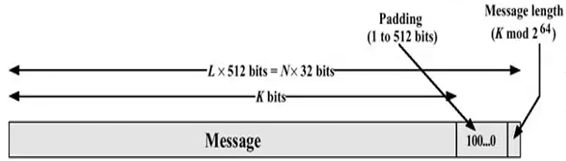
\includegraphics[width = 0.8 \textwidth]{padding.png}
\end{figure}
\subsubsection{Step 3: Initialize MD Buffer}
用一个128位的缓冲区来存储中间结果和最终结果。这个128位缓冲使用4个32位的寄存器$P,Q,R,S$实现。缓冲区被初始化为:
$$
    \begin{aligned}
        P= & 01,23,45,67 \\
        Q= & 89,AB,CD,EF \\
        R= & FE,DC,BA,98 \\
        S= & 76,54,32,10
    \end{aligned}
$$
初始值也被称为$IV$(initial values)。
\subsubsection{Step 4: Process Message in 512-bit blocks}
如图进行4轮处理:
\begin{figure}[H]
    \centering
    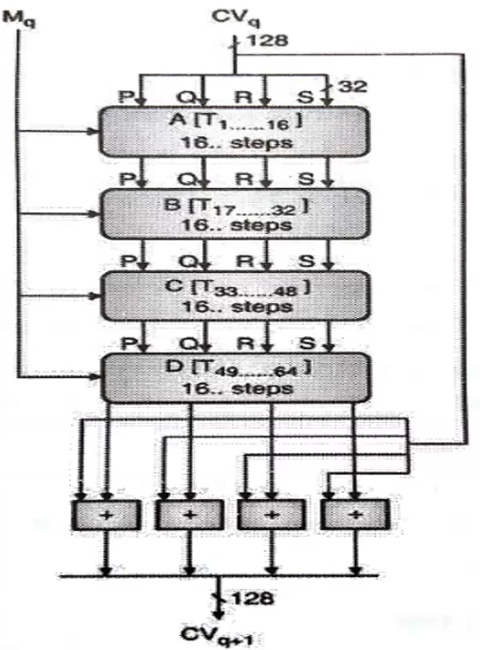
\includegraphics[width = 0.3 \textwidth]{ABCD.png}
\end{figure}
这四轮有和SHA类似的结构,但是在逻辑函数原语$A,B,C,D$有所不同
每一轮接收512位的块,处理并产生128位输出,第4轮128位输出加上$CV_q$(current values)产生$CV_{q+1}$。
\subsubsection{Step 5: Output}
在处理完全部$L$个块后,最后产生的128位消息摘要作为输出。
\begin{figure}[H]
    \centering
    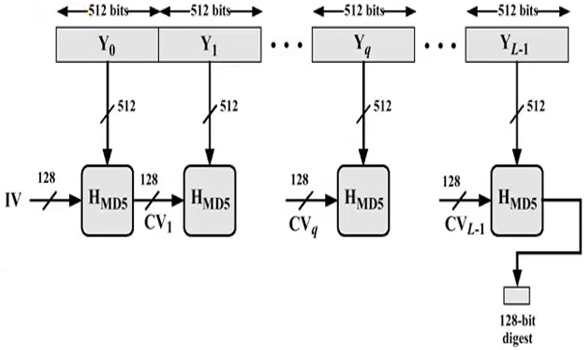
\includegraphics[width = 0.8 \textwidth]{whole.png}
\end{figure}
\subsection{MD5碰撞}
王小云、于洪波在2005年发表的文章描述了一种算法,来找到一对不同的数据拥有相同的MD5哈希值。其中一对著名的数据对分别是:
\begin{lstlisting}
d131dd02c5e6eec4693d9a0698aff95c2fcab58712467eab4004583eb8fb7f89 
55ad340609f4b30283e488832571415a085125e8f7cdc99fd91dbdf280373c5b 
d8823e3156348f5bae6dacd436c919c6dd53e2b487da03fd02396306d248cda0 
e99f33420f577ee8ce54b67080a80d1ec69821bcb6a8839396f9652b6ff72a70
\end{lstlisting}
和
\begin{lstlisting}
d131dd02c5e6eec4693d9a0698aff95c2fcab58712467eab4004583eb8fb7f89 
55ad340609f4b30283e488832571415a085125e8f7cdc99fd91dbdf280373c5b 
d8823e3156348f5bae6dacd436c919c6dd53e2b487da03fd02396306d248cda0 
e99f33420f577ee8ce54b67080a80d1ec69821bcb6a8839396f9652b6ff72a70
\end{lstlisting}
它们的MD5哈希值都是
\begin{lstlisting}
79054025255fb1a26e4bc422aef54eb4
\end{lstlisting}
假设$f$就是前面提到的A、B、C、D四个步骤,王小云和于洪波提出的方法,对于任意给定的$CV_q$,都可以实现找到四个块$M,M',N,N'$使得,有$f(f(CV_q,M),M')=f(f(CV_q,N),N')$。
非常重要的一点在于由于$CV_q$是任意的,我们可以基于此构造出任意的碰撞的数据。这样就说明MD5是不满足碰撞抗性的。运用这个方法可以构造一些有实际意义的攻击,比如利用分支结构:
\begin{lstlisting}
Program 1: if (data1 == data1) then { good_program } else { evil_program }
\end{lstlisting}
\begin{lstlisting}
Program 2: if (data2 == data1) then { good_program } else { evil_program }
\end{lstlisting}

\section{实验}
\subsection{创建两个碰撞的文件}
运行write.py创建二进制文件a、b,分别为:
\begin{lstlisting}
d131dd02c5e6eec4693d9a0698aff95c2fcab58712467eab4004583eb8fb7f89 
55ad340609f4b30283e488832571415a085125e8f7cdc99fd91dbdf280373c5b 
d8823e3156348f5bae6dacd436c919c6dd53e2b487da03fd02396306d248cda0 
e99f33420f577ee8ce54b67080a80d1ec69821bcb6a8839396f9652b6ff72a70
\end{lstlisting}
\begin{figure}[H]
    \centering
    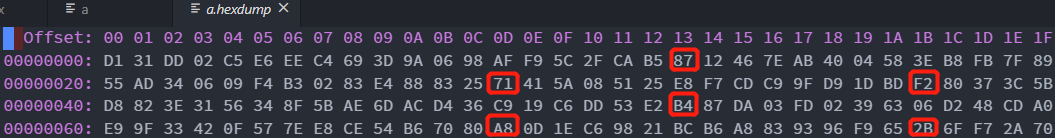
\includegraphics[width = \textwidth]{a.png}
\end{figure}
和
\begin{lstlisting}
d131dd02c5e6eec4693d9a0698aff95c2fcab58712467eab4004583eb8fb7f89 
55ad340609f4b30283e488832571415a085125e8f7cdc99fd91dbdf280373c5b 
d8823e3156348f5bae6dacd436c919c6dd53e2b487da03fd02396306d248cda0 
e99f33420f577ee8ce54b67080a80d1ec69821bcb6a8839396f9652b6ff72a70
\end{lstlisting}
\begin{figure}[H]
    \centering
    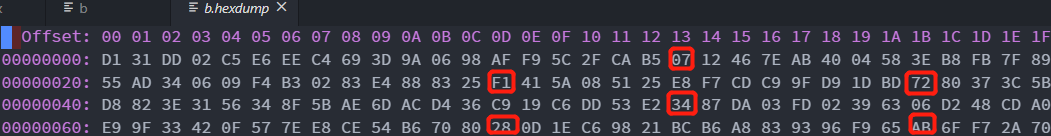
\includegraphics[width = \textwidth]{b.png}
\end{figure}
使用编译md5.c生成的md5.exe计算其哈希值:
\begin{figure}[H]
    \centering
    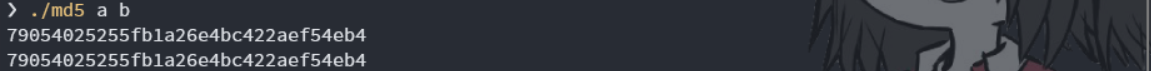
\includegraphics[width = \textwidth]{hash_a_b.png}
\end{figure}
发现两个不同的数据哈希值是一样的,都是:
\begin{lstlisting}
79054025255fb1a26e4bc422aef54eb4
\end{lstlisting}
\subsection{利用MD5碰撞实现攻击}
先使用NASM语法编写hello\_world\_raw.asm,其中包括分支结构:
\begin{lstlisting}
loop:
    mov cl, [data1+bx]
    cmp cl, [data2+bx]
    jnz evil
    inc bx
    cmp bx, 0x80
    jz good
    jmp loop
\end{lstlisting}
在data1、data2前面补充0,使其前面长度是512位即64比特的倍数:
\begin{lstlisting}
times 0x80-($-$$) db 0
\end{lstlisting}
将data1、data2全部初始化为0(为了确保data1、data2的位置正确,以保证可以正确利用其标签):
\begin{lstlisting}
data1: times 0x80-($-$$) db 0
data2: times 0x80-($-$$) db 0
\end{lstlisting}
编译hello\_world.asm,得hello\_world\_raw.com:
\begin{figure}[H]
    \centering
    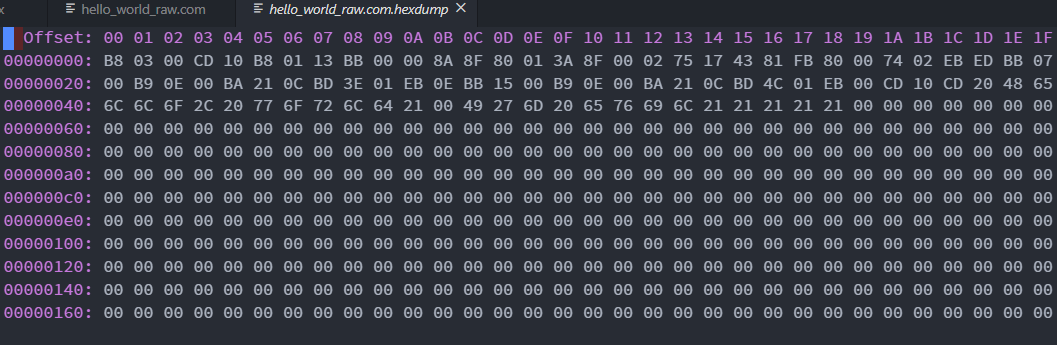
\includegraphics[width = \textwidth]{raw.png}
\end{figure}
运行delete.py把hello\_world\_raw.com的data1、data2去掉,以留出位置给真正的data1、data2,生成新文件叫hello\_world.com:
\begin{figure}[H]
    \centering
    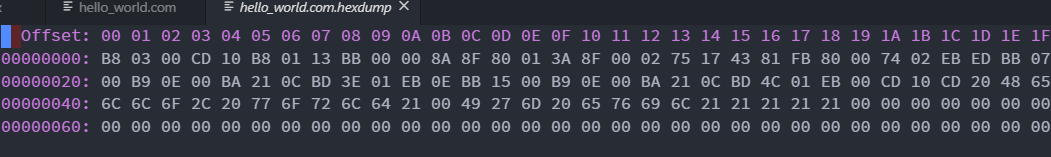
\includegraphics[width = \textwidth]{hello.png}
\end{figure}
使用下载的工具fastcoll.exe在hello\_world.com后加后缀,快速生成两个不同的,哈希值却相同的文件hello\_world\_msg1.com,hello\_world\_msg2.com:
\begin{figure}[H]
    \centering
    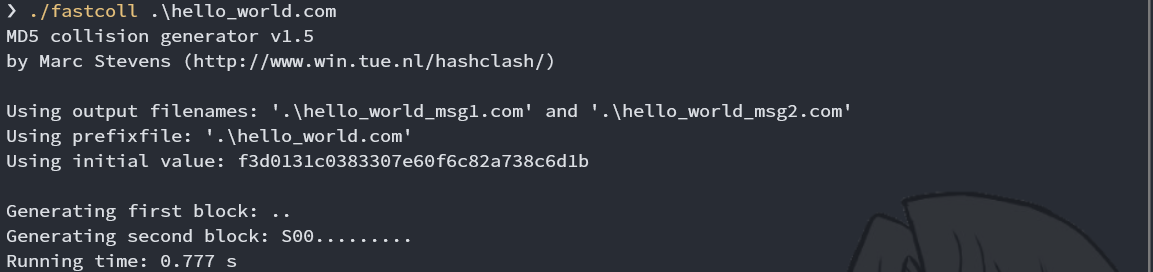
\includegraphics[width = \textwidth]{fastcoll.png}
\end{figure}
\begin{figure}[H]
    \centering
    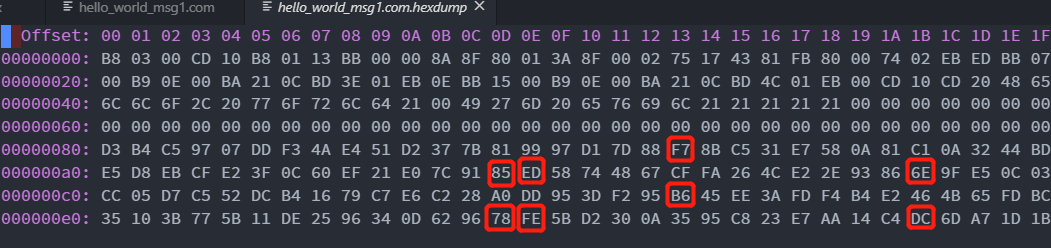
\includegraphics[width = \textwidth]{msg1.png}
\end{figure}
\begin{figure}[H]
    \centering
    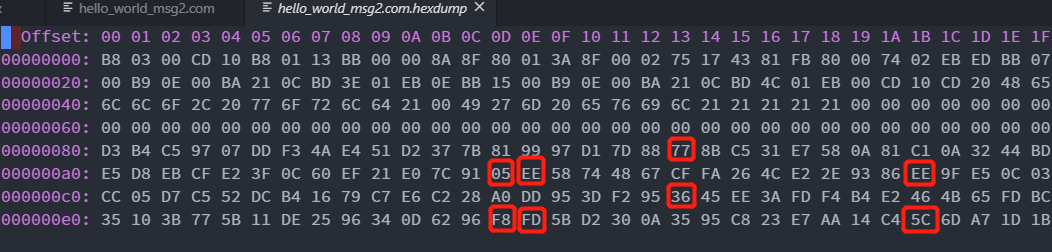
\includegraphics[width = \textwidth]{msg2.png}
\end{figure}
运行datacopy.py把msg1的data1复制到msg1和msg2的data2的位置,且分别重命名成good.com和evil.com:
\begin{figure}[H]
    \centering
    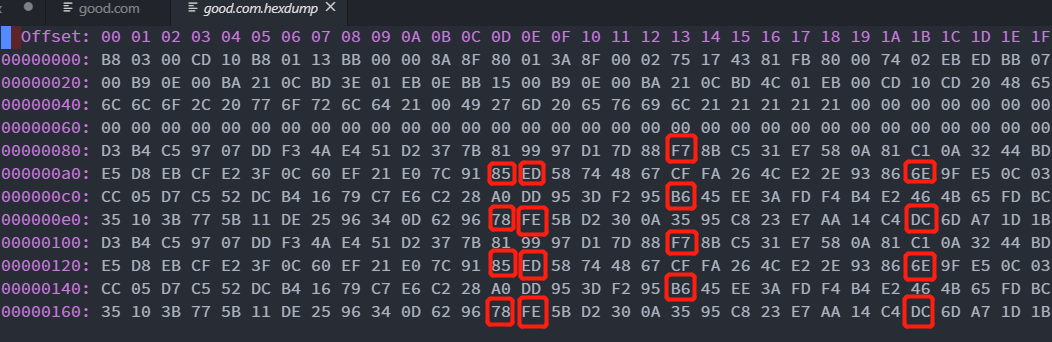
\includegraphics[width = \textwidth]{good_hex.png}
\end{figure}
\begin{figure}[H]
    \centering
    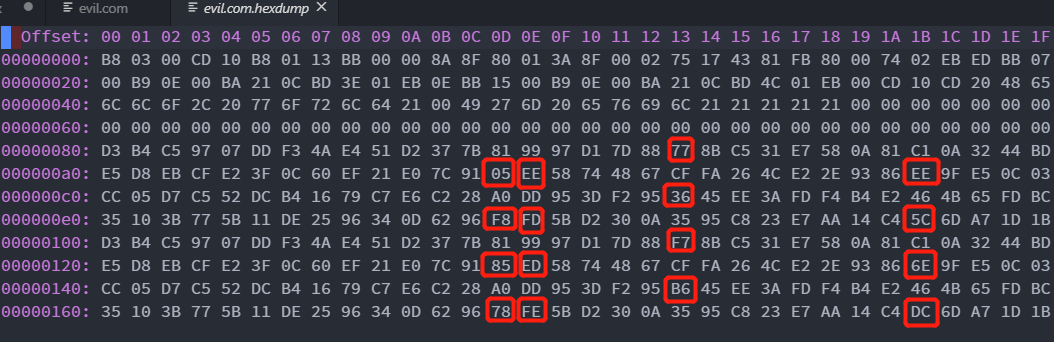
\includegraphics[width = \textwidth]{evil_hex.png}
\end{figure}
使用dosbox(或其他dos模拟器)运行good.com和evil.com:
\begin{figure}[H]
    \centering
    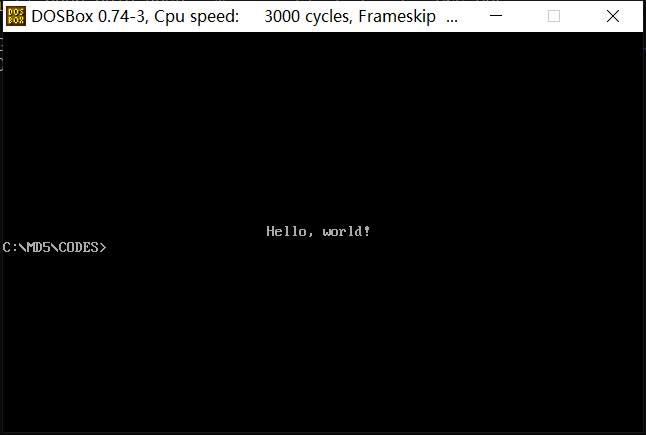
\includegraphics[width = 0.9\textwidth]{good.png}
\end{figure}
\begin{figure}[H]
    \centering
    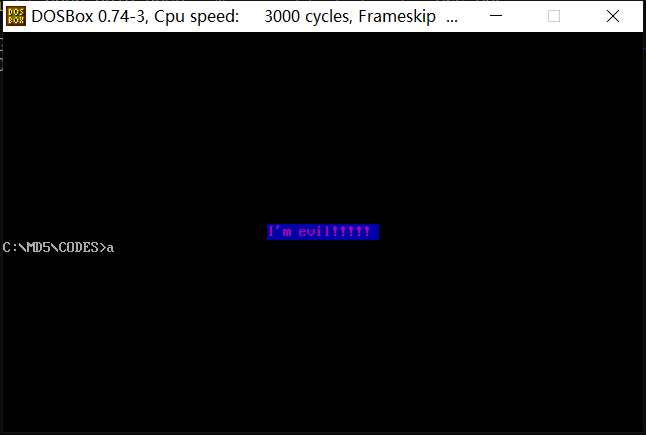
\includegraphics[width = 0.9\textwidth]{evil.png}
\end{figure}
使用md5.exe查看两个文件的哈希值:
\begin{figure}[H]
    \centering
    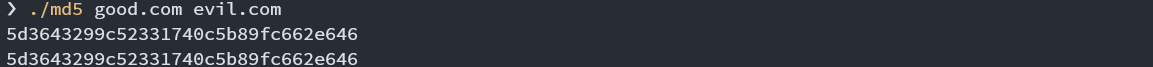
\includegraphics[width = \textwidth]{md5.png}
\end{figure}

\subsection{MD5实现随机数}
使用python实现,md5使用python库,实现md5rand.py如下:
\begin{lstlisting}
from hashlib import md5
import matplotlib.pyplot as plt


domain = 10
sample = 1000000


y = [0] * domain
for i in range(sample):
    y[int(md5(i.to_bytes(64, "little")).hexdigest(), 16) % domain] += 1
plt.bar(range(domain), y)
plt.show()
\end{lstlisting}
每次采样生成0-9的随机整数,总共采样1000000次,最终采样结果:
\begin{figure}[H]
    \centering
    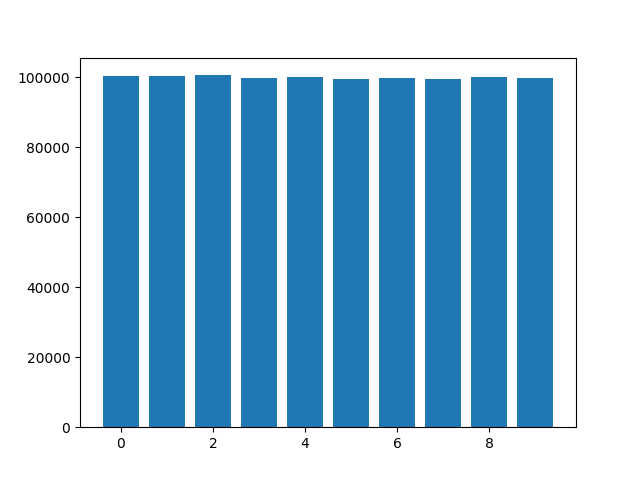
\includegraphics[width = \textwidth]{rand.png}
\end{figure}
\section{感想}
利用MD5碰撞可以轻易发动危害比较大的攻击,而碰撞攻击在三种攻击中的危害却又是最小的,因而可见哈希函数的安全性分析是非常重要的。另外MD5虽然已经多次被证明是不安全的哈希函数,但是仍可以
应用于一些对安全性要求不高的场景,如随机整数生成。因此MD5作为一个哈希函数在一些场景下并没有过时。

%\clearpage
%\bibliography{E:/Papers/LiuLab}
%\bibliographystyle{apalike}
\end{document}
%%% Local Variables:
%%% mode: latex
%%% TeX-master: t
%%% End:
